%%%%%%%%%%%%%%%%%%%%%%%%%%%%%%%%%%%%%%%%%%%%%%%%%%%%%%%%%%%%%%%%%%%%%%%
%%%
%%%         【非公式】東京理科大学 創域理工学部 機械航空宇宙工学科
%%%                       卒業論文要旨 テンプレート
%%%
%%%                                  v1.3.0 Yuki MATSUKAWA 01 Feb. 2023
%%%                                  v2.0.0 Yuki MATSUKAWA 14 Dec. 2023
%%%
%%%%%%%%%%%%%%%%%%%%%%%%%%%%%%%%%%%%%%%%%%%%%%%%%%%%%%%%%%%%%%%%%%%%%%%
\documentclass[a4paper,fleqn,dvipdfmx,12pt]{jreport}

%%% abstract style %%%
\usepackage{bachelor_settings}
\usepackage{epsf,color}
\usepackage{float}
\usepackage{subfigure}
\usepackage{rotating}
\usepackage{lscape}
\usepackage{bm}
\usepackage{multirow}
\usepackage{multicol}

% ページ番号を付けない
\pagestyle{empty}

\begin{document}

%%%%%%%%%%%%%%%%%
%%% 日本語要旨 %%%
%%%%%%%%%%%%%%%%%

\begin{center}
\fontsize{16pt}{16pt}\selectfont
{\gtfamily\bfseries 
% 卒業論文の日本語題目
ここには卒業論文のタイトルを入れます.\\ 一文字でも間違えたら受理されません.
% 卒業論文の日本語題目
}
\end{center}

\noindent
% 学籍番号,姓,名の間に「全角」スペース忘れずに
% xx を研究室名に変更
% \hfill は消さない
[xx研究室] \hfill 75***** 姓姓 名名

\vskip\baselineskip
\fontsize{12pt}{16pt}\selectfont
%%% ここから書き始める %%%
アブストラクトアブストラクトアブストラクトアブストラクトアブストラクトアブストラクトアブストラクトアブストラクトアブストラクト
アブストラクトアブストラクトアブストラクトアブストラクトアブストラクトアブストラクトアブストラクトアブストラクトアブストラクト
アブストラクトアブストラクトアブストラクトアブストラクトアブストラクトアブストラクトアブストラクトアブストラクトアブストラクト
アブストラクトアブストラクトアブストラクトアブストラクトアブストラクトアブストラクトアブストラクトアブストラクトアブストラクト
アブストラクトアブストラクトアブストラクトアブストラクトアブストラクトアブストラクトアブストラクトアブストラクトアブストラクト
アブストラクトアブストラクトアブストラクトアブストラクトアブストラクトアブストラクトアブストラクトアブストラクトアブストラクト
アブストラクトアブストラクトアブストラクトアブストラクトアブストラクトアブストラクトアブストラクトアブストラクトアブストラクト.

図~\ref{fig:abst1}は虎,図~\ref{fig:abst2}も虎.
アブストラクトアブストラクトアブストラクトアブストラクトアブストラクトアブストラクトアブストラクトアブストラクトアブストラクト
アブストラクトアブストラクトアブストラクトアブストラクトアブストラクトアブストラクトアブストラクトアブストラクトアブストラクト
アブストラクトアブストラクトアブストラクトアブストラクトアブストラクトアブストラクトアブストラクトアブストラクトアブストラクト
アブストラクトアブストラクトアブストラクトアブストラクトアブストラクトアブストラクトアブストラクトアブストラクトアブストラクト
アブストラクトアブストラクトアブストラクトアブストラクトアブストラクトアブストラクトアブストラクトアブストラクトアブストラクト
アブストラクトアブストラクトアブストラクトアブストラクトアブストラクトアブストラクトアブストラクトアブストラクトアブストラクト
アブストラクトアブストラクトアブストラクトアブストラクトアブストラクトアブストラクトアブストラクトアブストラクトアブストラクト
アブストラクトアブストラクトアブストラクトアブストラクトアブストラクトアブストラクトアブストラクトアブストラクトアブストラクト
アブストラクトアブストラクトアブストラクトアブストラクトアブストラクトアブストラクトアブストラクトアブストラクトアブストラクト
アブストラクトアブストラクトアブストラクトアブストラクトアブストラクトアブストラクトアブストラクトアブストラクトアブストラクト
アブストラクトアブストラクトアブストラクトアブストラクトアブストラクトアブストラクトアブストラクトアブストラクトアブストラクト.

\begin{multicols}{2}
   	\begin{figure}[H]
   		\centering
   		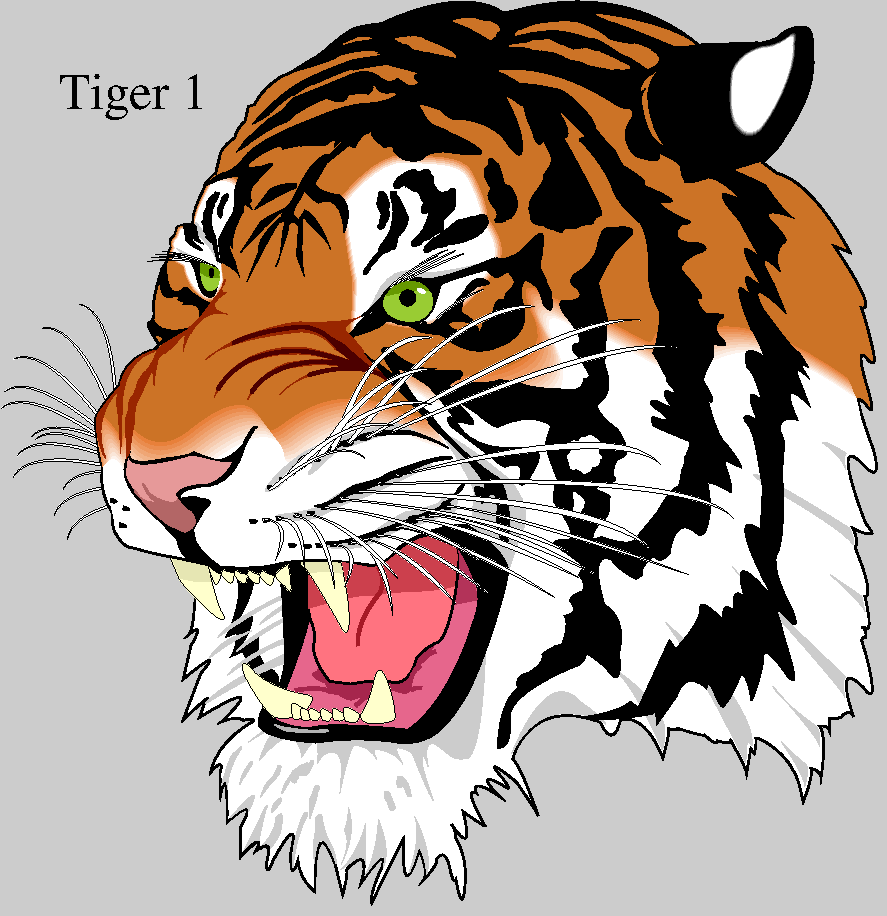
\includegraphics[width=0.6\columnwidth]{tiger_1.pdf}
   		\caption{Tiger 1.}
   		\label{fig:abst1}
   	\end{figure}

   	\begin{figure}[H]
		\centering
   		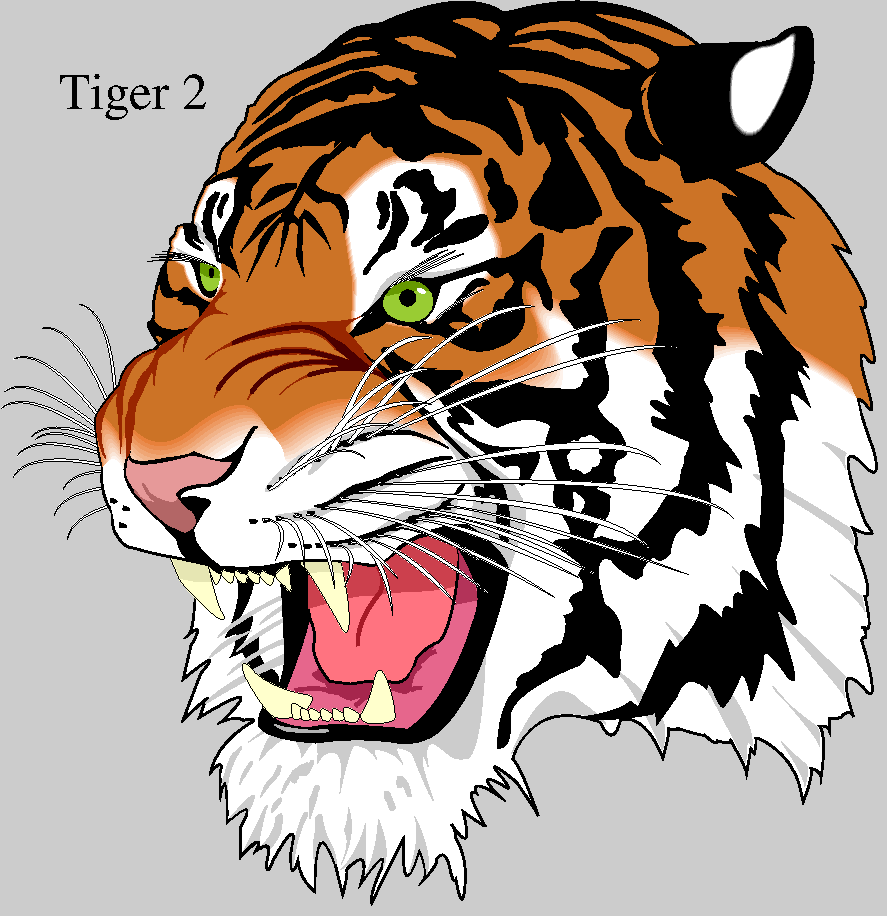
\includegraphics[width=0.6\columnwidth]{tiger_2.pdf}
   		\caption{Tiger 2.}
   		\label{fig:abst2}
   	\end{figure}
\end{multicols}

%%% ここまで %%%

%%% ここで改ページ %%%
\clearpage

%%%%%%%%%%%%%%%%%
%%%% 英語要旨 %%%%
%%%%%%%%%%%%%%%%%

\begin{center}
{\sffamily\bfseries 
% 卒業論文の英語題目
Enter the title of your graduation thesis here. \\ If you make a mistake in even one letter, it will not be accepted.
% 卒業論文の英語題目
}
\end{center}

\noindent
% 氏名の大文字小文字に注意(名は冒頭のみ大文字,姓は全て大文字)
% 学籍番号,名,姓の間に「半角」スペース忘れずに
% xx を研究室名に変更
% \hfill は消さない
[xx Group] \hfill 75***** First FAMILY

\vskip\baselineskip
%%% ここから書き始める %%%
Abstract abstract abstract abstract abstract abstract abstract abstract abstract 
abstract abstract abstract abstract abstract abstract abstract abstract abstract
abstract abstract abstract abstract abstract abstract abstract abstract abstract
abstract abstract abstract abstract abstract abstract abstract abstract abstract
abstract abstract abstract abstract abstract abstract abstract abstract abstract
abstract abstract abstract abstract abstract abstract abstract abstract abstract
abstract abstract abstract abstract abstract abstract abstract abstract abstract
abstract abstract abstract abstract abstract abstract abstract abstract abstract.

%%% ここまで %%%

\end{document}